% Options for packages loaded elsewhere
% Options for packages loaded elsewhere
\PassOptionsToPackage{unicode}{hyperref}
\PassOptionsToPackage{hyphens}{url}
%
\documentclass[
  english,
  russian,
  12pt,
  a4paper,
  DIV=11,
  numbers=noendperiod]{scrreprt}
\usepackage{xcolor}
\usepackage{amsmath,amssymb}
\setcounter{secnumdepth}{5}
\usepackage{iftex}
\ifPDFTeX
  \usepackage[T1]{fontenc}
  \usepackage[utf8]{inputenc}
  \usepackage{textcomp} % provide euro and other symbols
\else % if luatex or xetex
  \usepackage{unicode-math} % this also loads fontspec
  \defaultfontfeatures{Scale=MatchLowercase}
  \defaultfontfeatures[\rmfamily]{Ligatures=TeX,Scale=1}
\fi
\usepackage{lmodern}
\ifPDFTeX\else
  % xetex/luatex font selection
\fi
% Use upquote if available, for straight quotes in verbatim environments
\IfFileExists{upquote.sty}{\usepackage{upquote}}{}
\IfFileExists{microtype.sty}{% use microtype if available
  \usepackage[]{microtype}
  \UseMicrotypeSet[protrusion]{basicmath} % disable protrusion for tt fonts
}{}
\usepackage{setspace}
% Make \paragraph and \subparagraph free-standing
\makeatletter
\ifx\paragraph\undefined\else
  \let\oldparagraph\paragraph
  \renewcommand{\paragraph}{
    \@ifstar
      \xxxParagraphStar
      \xxxParagraphNoStar
  }
  \newcommand{\xxxParagraphStar}[1]{\oldparagraph*{#1}\mbox{}}
  \newcommand{\xxxParagraphNoStar}[1]{\oldparagraph{#1}\mbox{}}
\fi
\ifx\subparagraph\undefined\else
  \let\oldsubparagraph\subparagraph
  \renewcommand{\subparagraph}{
    \@ifstar
      \xxxSubParagraphStar
      \xxxSubParagraphNoStar
  }
  \newcommand{\xxxSubParagraphStar}[1]{\oldsubparagraph*{#1}\mbox{}}
  \newcommand{\xxxSubParagraphNoStar}[1]{\oldsubparagraph{#1}\mbox{}}
\fi
\makeatother


\usepackage{longtable,booktabs,array}
\usepackage{calc} % for calculating minipage widths
% Correct order of tables after \paragraph or \subparagraph
\usepackage{etoolbox}
\makeatletter
\patchcmd\longtable{\par}{\if@noskipsec\mbox{}\fi\par}{}{}
\makeatother
% Allow footnotes in longtable head/foot
\IfFileExists{footnotehyper.sty}{\usepackage{footnotehyper}}{\usepackage{footnote}}
\makesavenoteenv{longtable}
\usepackage{graphicx}
\makeatletter
\newsavebox\pandoc@box
\newcommand*\pandocbounded[1]{% scales image to fit in text height/width
  \sbox\pandoc@box{#1}%
  \Gscale@div\@tempa{\textheight}{\dimexpr\ht\pandoc@box+\dp\pandoc@box\relax}%
  \Gscale@div\@tempb{\linewidth}{\wd\pandoc@box}%
  \ifdim\@tempb\p@<\@tempa\p@\let\@tempa\@tempb\fi% select the smaller of both
  \ifdim\@tempa\p@<\p@\scalebox{\@tempa}{\usebox\pandoc@box}%
  \else\usebox{\pandoc@box}%
  \fi%
}
% Set default figure placement to htbp
\def\fps@figure{htbp}
\makeatother



\ifLuaTeX
\usepackage[bidi=basic,provide=*]{babel}
\else
\usepackage[bidi=default,provide=*]{babel}
\fi
% get rid of language-specific shorthands (see #6817):
\let\LanguageShortHands\languageshorthands
\def\languageshorthands#1{}


\setlength{\emergencystretch}{3em} % prevent overfull lines

\providecommand{\tightlist}{%
  \setlength{\itemsep}{0pt}\setlength{\parskip}{0pt}}



 
\usepackage[style=gost-numeric,backend=biber,langhook=extras,autolang=other*]{biblatex}
\addbibresource{bib/cite.bib}

\usepackage[]{csquotes}

\usepackage{indentfirst}
\usepackage{float}
\floatplacement{figure}{H}
\IfFileExists{plex-otf.sty}{
  %% Full TeXlive
  \usepackage[
    % math,
    RM={Scale=0.94},SS={Scale=0.94},SScon={Scale=0.94},TT={Scale=MatchLowercase,FakeStretch=0.9},
    DefaultFeatures={Ligatures=Common}
  ]{plex-otf}
  % \usepackage[Scale=MatchUppercase]{juliamono}
}{
  %% TinyTeX
  \usepackage{libertine}
}
\KOMAoption{captions}{tableheading}
\makeatletter
\@ifpackageloaded{caption}{}{\usepackage{caption}}
\AtBeginDocument{%
\ifdefined\contentsname
  \renewcommand*\contentsname{Содержание}
\else
  \newcommand\contentsname{Содержание}
\fi
\ifdefined\listfigurename
  \renewcommand*\listfigurename{Список иллюстраций}
\else
  \newcommand\listfigurename{Список иллюстраций}
\fi
\ifdefined\listtablename
  \renewcommand*\listtablename{Список таблиц}
\else
  \newcommand\listtablename{Список таблиц}
\fi
\ifdefined\figurename
  \renewcommand*\figurename{Рисунок}
\else
  \newcommand\figurename{Рисунок}
\fi
\ifdefined\tablename
  \renewcommand*\tablename{Таблица}
\else
  \newcommand\tablename{Таблица}
\fi
}
\@ifpackageloaded{float}{}{\usepackage{float}}
\floatstyle{ruled}
\@ifundefined{c@chapter}{\newfloat{codelisting}{h}{lop}}{\newfloat{codelisting}{h}{lop}[chapter]}
\floatname{codelisting}{Список}
\newcommand*\listoflistings{\listof{codelisting}{Листинги}}
\makeatother
\makeatletter
\makeatother
\makeatletter
\@ifpackageloaded{caption}{}{\usepackage{caption}}
\@ifpackageloaded{subcaption}{}{\usepackage{subcaption}}
\makeatother
\usepackage{bookmark}
\IfFileExists{xurl.sty}{\usepackage{xurl}}{} % add URL line breaks if available
\urlstyle{same}
\hypersetup{
  pdftitle={Отчёт по лабораторной работе №9},
  pdfauthor={Абу Зейтун Саед Фатхи Бадер},
  pdflang={ru-RU},
  hidelinks,
  pdfcreator={LaTeX via pandoc}}


\title{Отчёт по лабораторной работе №9}
\usepackage{etoolbox}
\makeatletter
\providecommand{\subtitle}[1]{% add subtitle to \maketitle
  \apptocmd{\@title}{\par {\large #1 \par}}{}{}
}
\makeatother
\subtitle{Командная оболочка Midnight Commander}
\author{Абу Зейтун Саед Фатхи Бадер}
\date{}
\begin{document}
\maketitle

\renewcommand*\contentsname{Содержание}
{
\setcounter{tocdepth}{1}
\tableofcontents
}
\listoffigures
\listoftables

\setstretch{1.5}
\chapter{Цель
работы}\label{ux446ux435ux43bux44c-ux440ux430ux431ux43eux442ux44b}

Освоение основных возможностей командной оболочки Midnight Commander.
Приобретение навыков практической работы по просмотру каталогов и
файлов; манипуляций с ними.

\chapter{Выполнение лабораторной
работы}\label{ux432ux44bux43fux43eux43bux43dux435ux43dux438ux435-ux43bux430ux431ux43eux440ux430ux442ux43eux440ux43dux43eux439-ux440ux430ux431ux43eux442ux44b}

1 Изучим информацию о mc при помощи справки man. Воспользуемся справкой
и узнаем что для того чтобы войти в командную оболочку мы должны ввести
в командной строке mc.

2 Запустим из командной строки mc.

\begin{figure}

{\centering 
\includegraphics[width=0.7\linewidth,height=0.7\textheight]{image/01.png}

}

\caption{Запуск mc}

\end{figure}%

3 Выполните несколько операций в mc, используя управляющие клавиши

\begin{figure}

{\centering 
\includegraphics[width=0.7\linewidth,height=0.7\textheight]{image/02.png}

}

\caption{Выделение}

\end{figure}%

\begin{figure}

{\centering 
\includegraphics[width=0.7\linewidth,height=0.7\textheight]{image/03.png}

}

\caption{Отмена}

\end{figure}%

\begin{figure}

{\centering 
\includegraphics[width=0.7\linewidth,height=0.7\textheight]{image/04.png}

}

\caption{Копирование}

\end{figure}%

\begin{figure}

{\centering 
\includegraphics[width=0.7\linewidth,height=0.7\textheight]{image/05.png}

}

\caption{Перемещение}

\end{figure}%

\begin{figure}

{\centering 
\includegraphics[width=0.7\linewidth,height=0.7\textheight]{image/06.png}

}

\caption{Информация}

\end{figure}%

4 Выполните основные команды меню левой панели.

\begin{figure}

{\centering 
\includegraphics[width=0.7\linewidth,height=0.7\textheight]{image/07.png}

}

\caption{Быстрый просмотр}

\end{figure}%

\begin{figure}

{\centering 
\includegraphics[width=0.7\linewidth,height=0.7\textheight]{image/08.png}

}

\caption{Информация}

\end{figure}%

\begin{figure}

{\centering 
\includegraphics[width=0.7\linewidth,height=0.7\textheight]{image/09.png}

}

\caption{Дерево каталогов}

\end{figure}%

5 Используя возможности подменю Файл , выполним:

\begin{figure}

{\centering 
\includegraphics[width=0.7\linewidth,height=0.7\textheight]{image/10.png}

}

\caption{Просмотр содержимого текстового файла}

\end{figure}%

\begin{figure}

{\centering 
\includegraphics[width=0.7\linewidth,height=0.7\textheight]{image/11.png}

}

\caption{Отредактируем содержимое текстового файла без сохранения
результатов}

\end{figure}%

\begin{figure}

{\centering 
\includegraphics[width=0.7\linewidth,height=0.7\textheight]{image/12.png}

}

\caption{Создание каталога}

\end{figure}%

\begin{figure}

{\centering 
\includegraphics[width=0.7\linewidth,height=0.7\textheight]{image/13.png}

}

\caption{Копирование в файлов в созданный каталог}

\end{figure}%

\begin{enumerate}
\def\labelenumi{\arabic{enumi}.}
\setcounter{enumi}{5}
\tightlist
\item
  С помощью соответствующих средств подменю Команда осуществите:
\end{enumerate}

\begin{figure}

{\centering 
\includegraphics[width=0.7\linewidth,height=0.7\textheight]{image/14.png}

}

\caption{Поиск файлов}

\end{figure}%

\begin{figure}

{\centering 
\includegraphics[width=0.7\linewidth,height=0.7\textheight]{image/15.png}

}

\caption{История команд}

\end{figure}%

\begin{figure}

{\centering 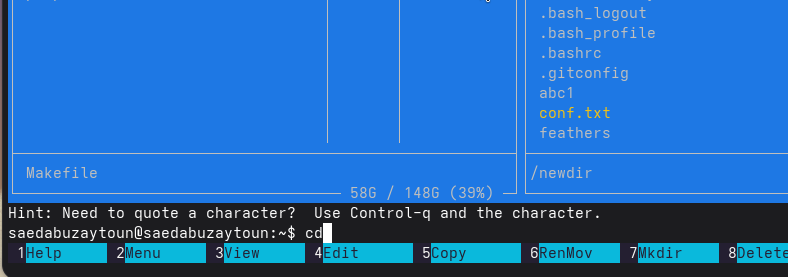
\includegraphics[width=0.7\linewidth,height=0.7\textheight]{image/16.png}

}

\caption{Переход в домашний каталог}

\end{figure}%

\begin{figure}

{\centering 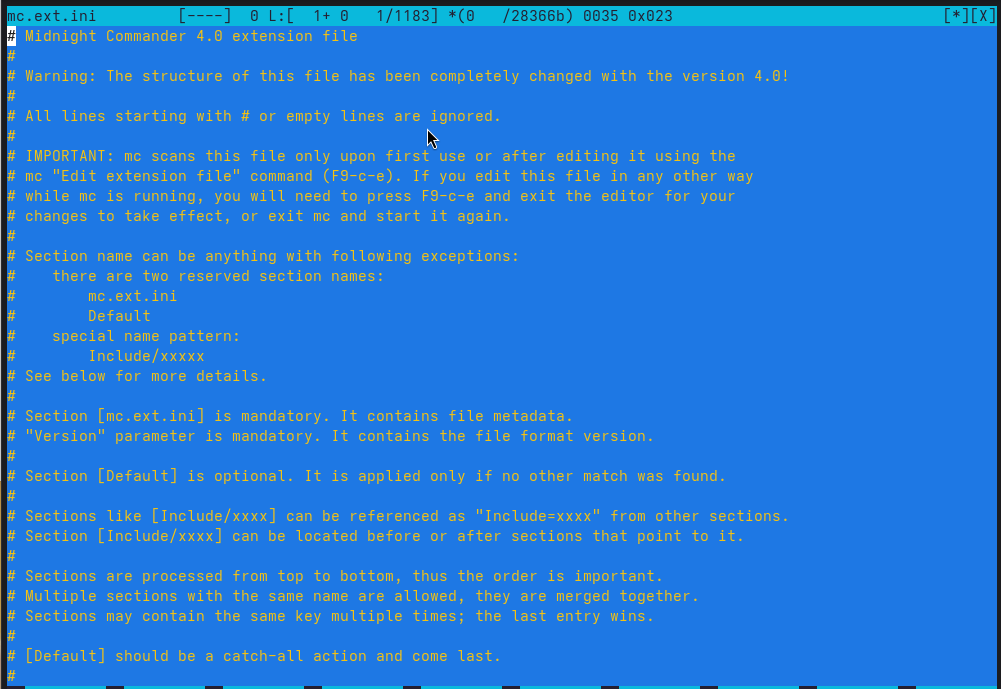
\includegraphics[width=0.7\linewidth,height=0.7\textheight]{image/17.png}

}

\caption{Просмотр файла расширений}

\end{figure}%

\begin{figure}

{\centering 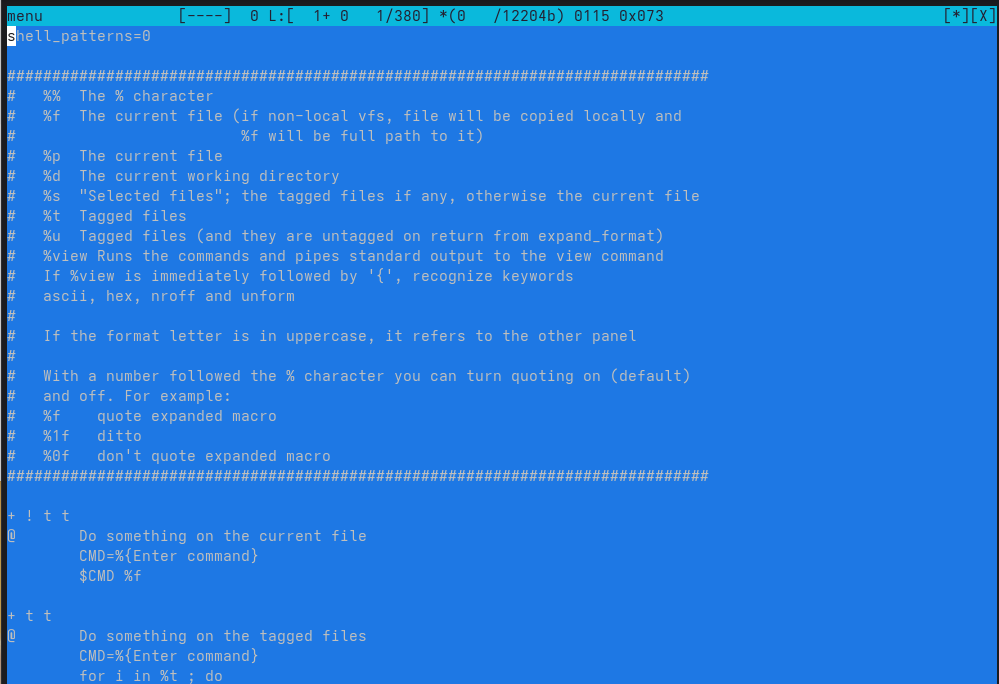
\includegraphics[width=0.7\linewidth,height=0.7\textheight]{image/18.png}

}

\caption{Просмотр файла меню}

\end{figure}%

\begin{enumerate}
\def\labelenumi{\arabic{enumi}.}
\setcounter{enumi}{6}
\tightlist
\item
  Вызовем подменю Настройки. Изучим опции
\end{enumerate}

\begin{figure}

{\centering 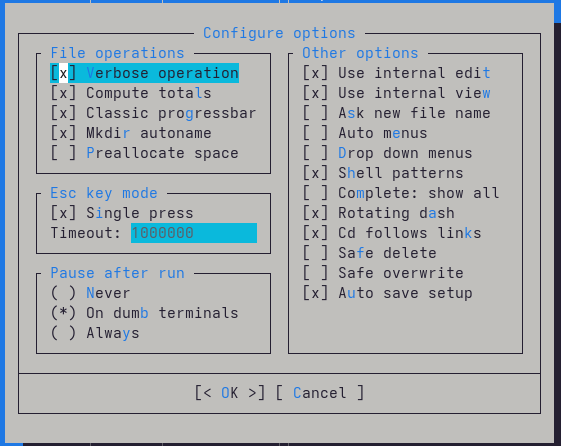
\includegraphics[width=0.7\linewidth,height=0.7\textheight]{image/19.png}

}

\caption{Конфигурация}

\end{figure}%

\begin{figure}

{\centering 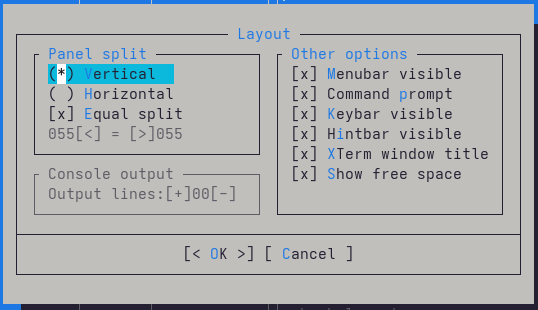
\includegraphics[width=0.7\linewidth,height=0.7\textheight]{image/20.png}

}

\caption{Внешний вид}

\end{figure}%

\begin{figure}

{\centering 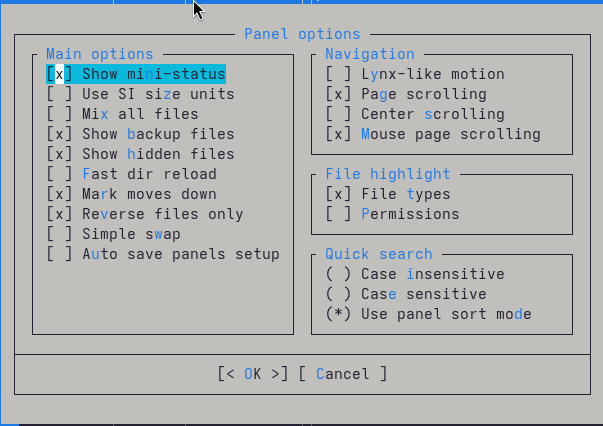
\includegraphics[width=0.7\linewidth,height=0.7\textheight]{image/21.png}

}

\caption{Настройки панелей}

\end{figure}%

\begin{figure}

{\centering 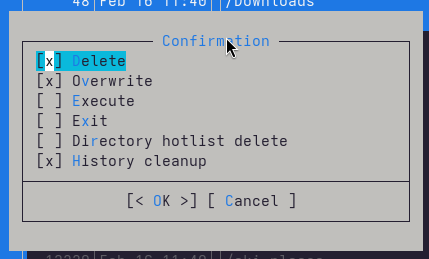
\includegraphics[width=0.7\linewidth,height=0.7\textheight]{image/22.png}

}

\caption{Подтверждение}

\end{figure}%

\begin{figure}

{\centering 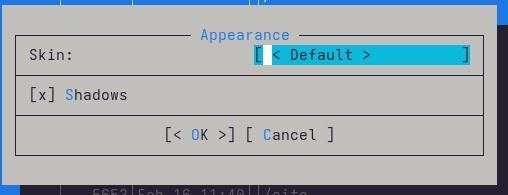
\includegraphics[width=0.7\linewidth,height=0.7\textheight]{image/23.png}

}

\caption{Оформление}

\end{figure}%

\begin{figure}

{\centering 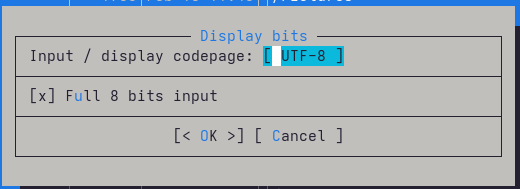
\includegraphics[width=0.7\linewidth,height=0.7\textheight]{image/24.png}

}

\caption{Кодировка символов}

\end{figure}%

\begin{figure}

{\centering 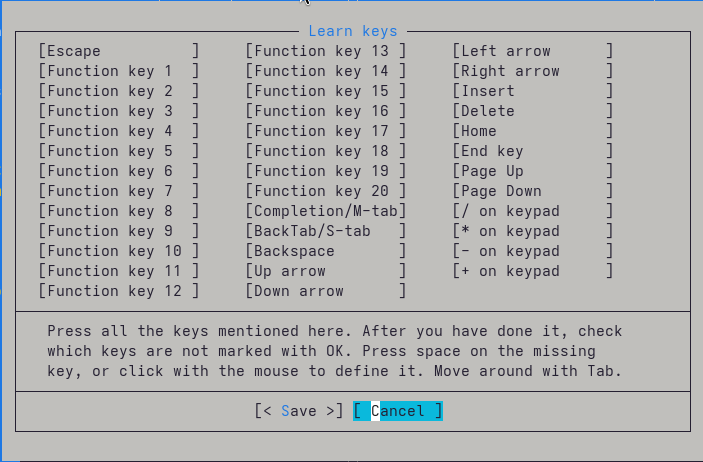
\includegraphics[width=0.7\linewidth,height=0.7\textheight]{image/25.png}

}

\caption{Распознавание клавиш}

\end{figure}%

8 Создадим текстовой файл text.txt.

9 Откроем этот файл с помощью встроенного в mc редактора, и вставим в
открытый файл небольшой фрагмент текста, скопированный из любого другого
файла или Интернета.

\begin{figure}

{\centering 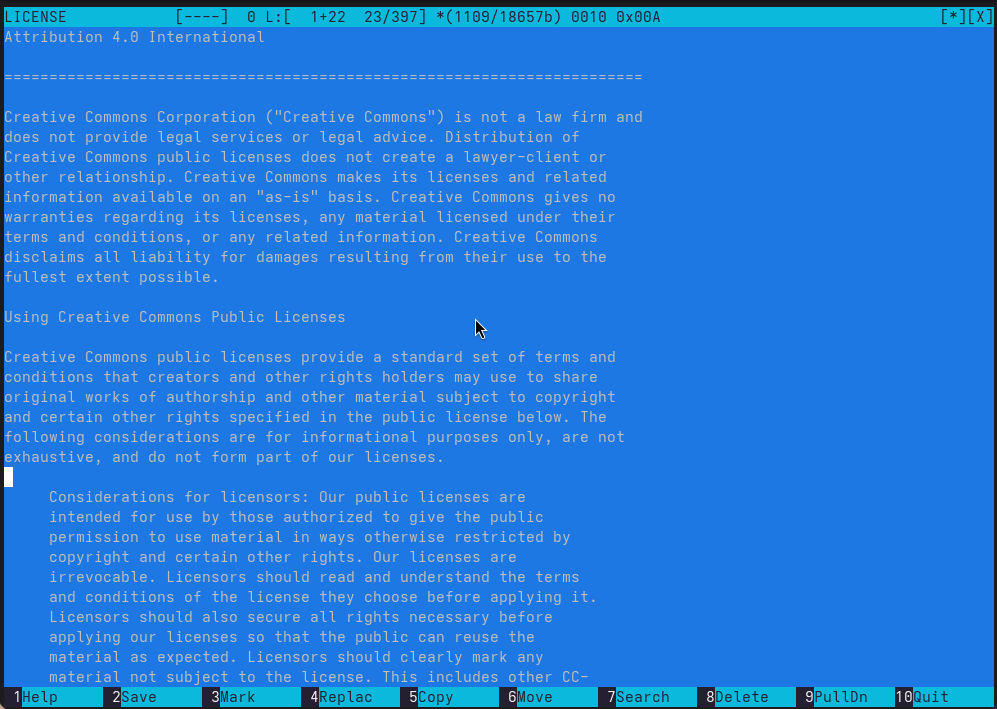
\includegraphics[width=0.7\linewidth,height=0.7\textheight]{image/26.png}

}

\caption{Файл с текстом}

\end{figure}%

10 Проделаем с текстом следующие манипуляции, используя горячие клавиши:

Удалим строку текста. - F8

\begin{figure}

{\centering 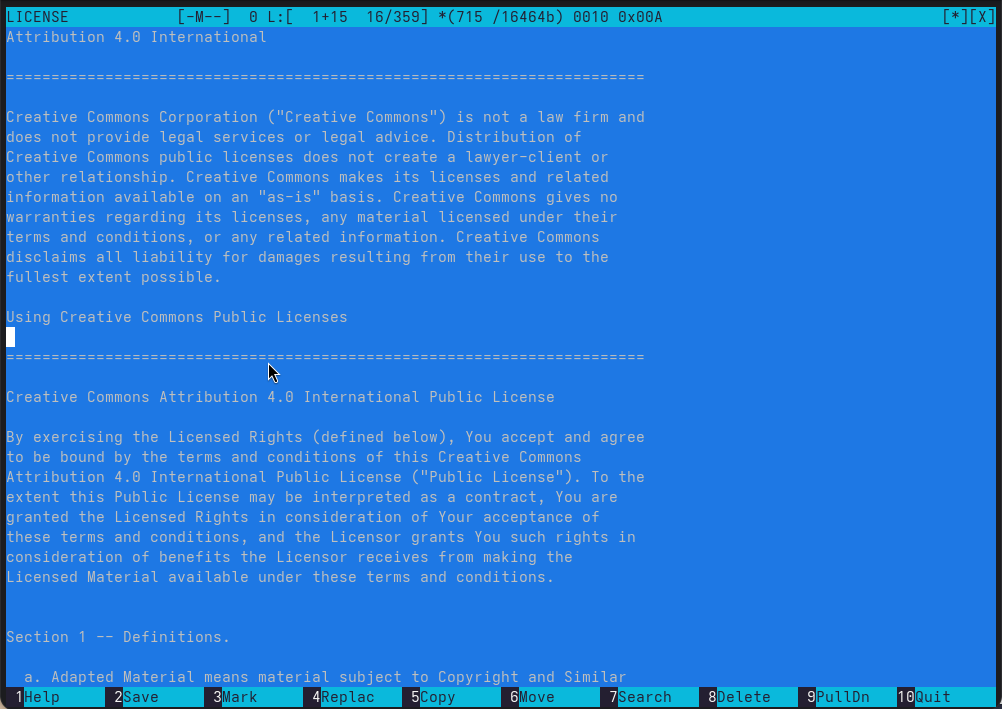
\includegraphics[width=0.7\linewidth,height=0.7\textheight]{image/27.png}

}

\caption{Файл с текстом}

\end{figure}%

Выделим фрагмент текста и скопируйте его на новую строку. - F5

\begin{figure}

{\centering 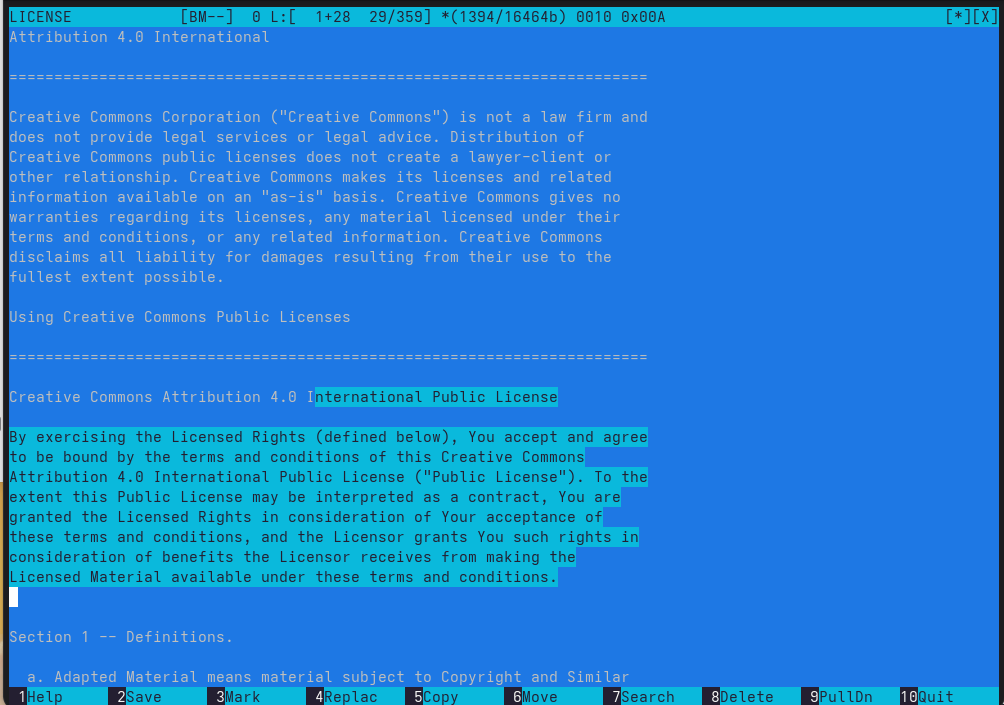
\includegraphics[width=0.7\linewidth,height=0.7\textheight]{image/28.png}

}

\caption{Копирование фрагмента}

\end{figure}%

Сохраним файл. - F2

\begin{figure}

{\centering 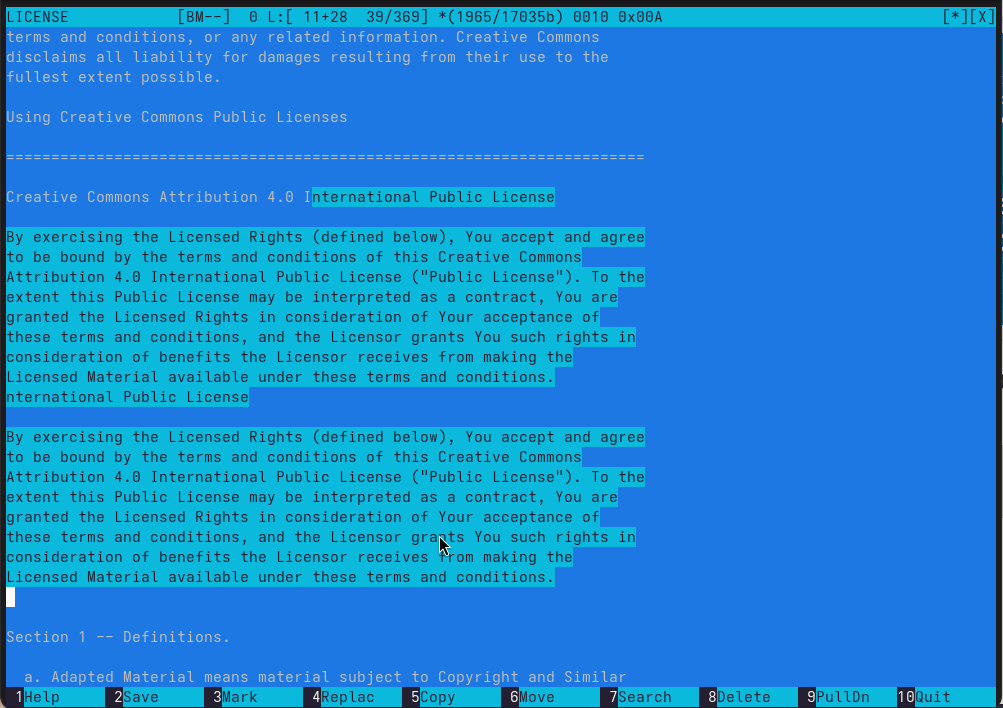
\includegraphics[width=0.7\linewidth,height=0.7\textheight]{image/29.png}

}

\caption{Сохранение}

\end{figure}%

Отменим последнее действие. - Ctrl+U

\begin{figure}

{\centering 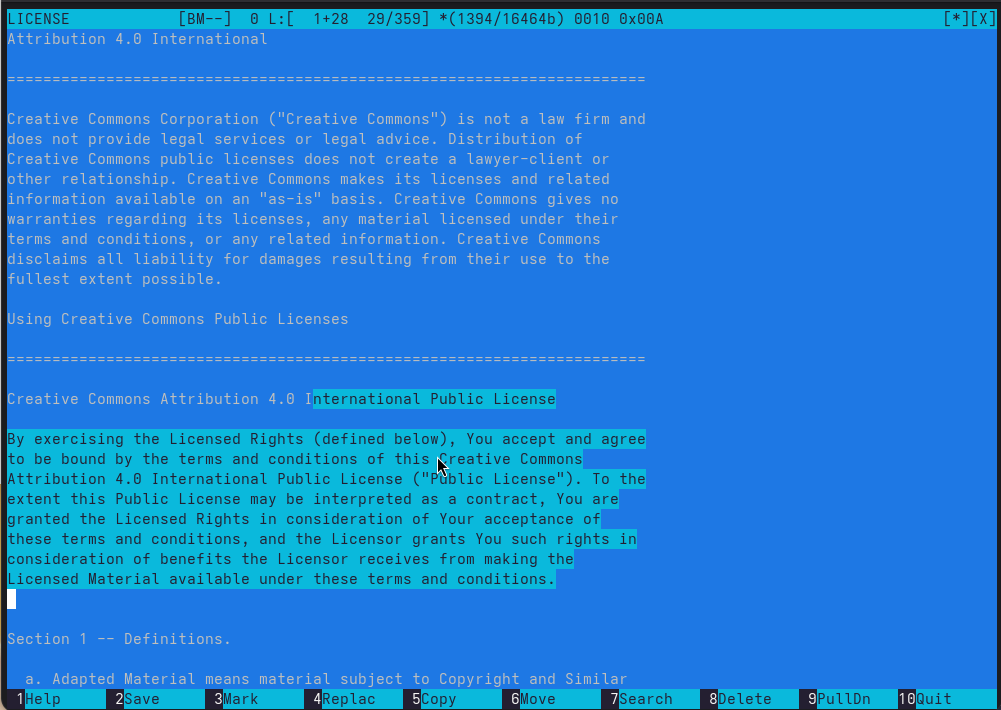
\includegraphics[width=0.7\linewidth,height=0.7\textheight]{image/30.png}

}

\caption{Отмена}

\end{figure}%

Перейдем в конец файла - PageDown или Ctrl+X

\begin{figure}

{\centering 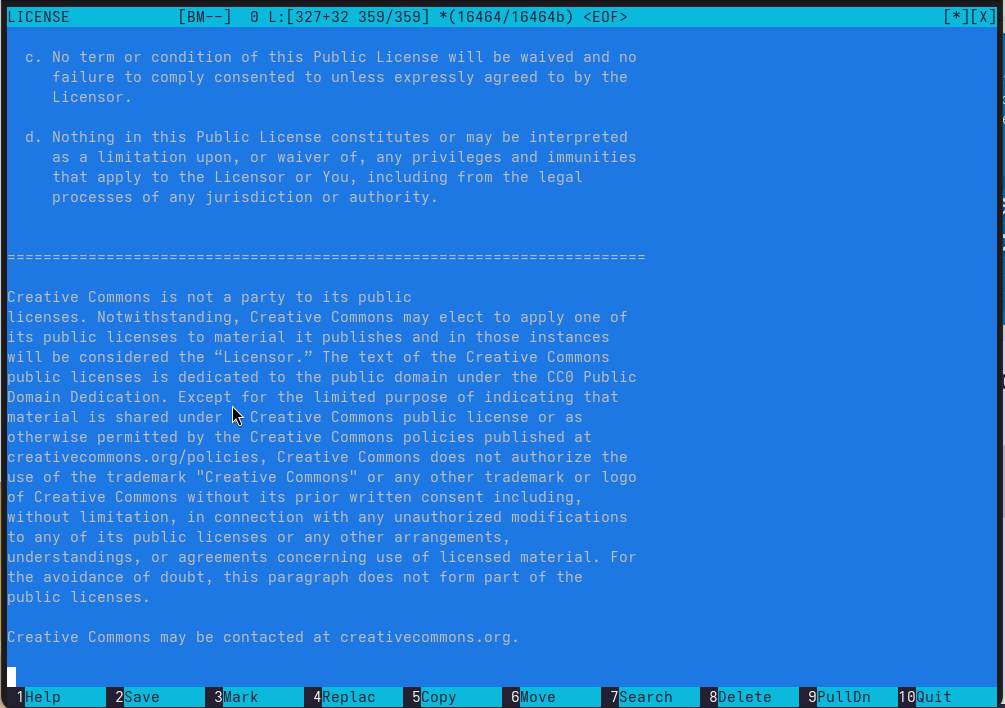
\includegraphics[width=0.7\linewidth,height=0.7\textheight]{image/31.png}

}

\caption{Переход в конец файла}

\end{figure}%

Перейдем в начало файла - PageUp или Ctrl+Z

\begin{figure}

{\centering 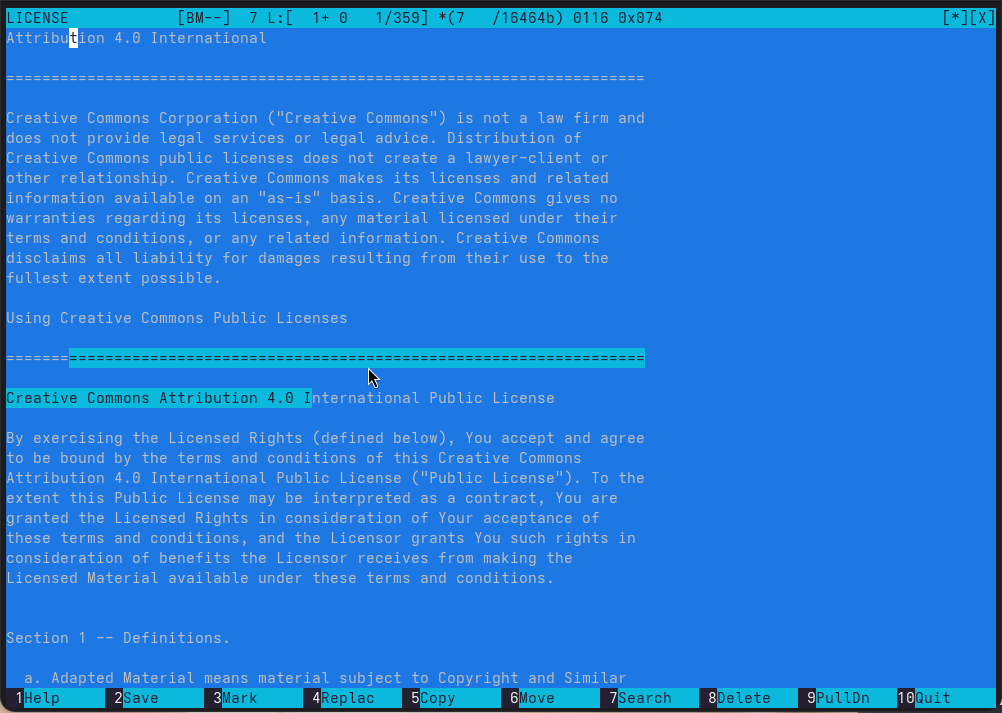
\includegraphics[width=0.7\linewidth,height=0.7\textheight]{image/32.png}

}

\caption{Переход в начало файла}

\end{figure}%

11 Откроем файл с исходным текстом на языке программирования C

\begin{figure}

{\centering 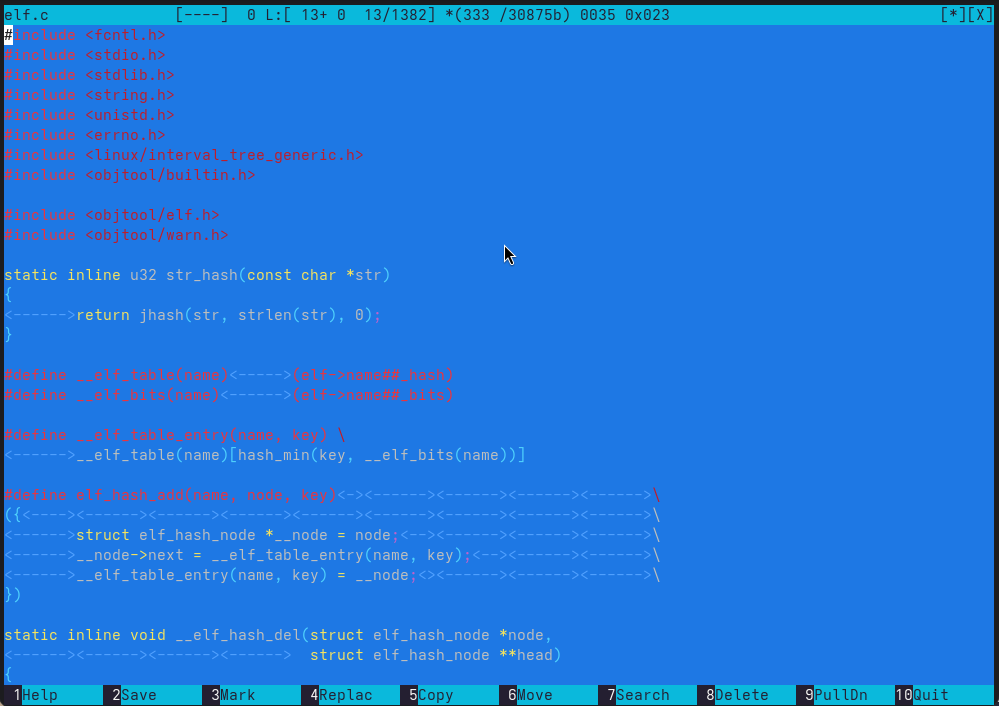
\includegraphics[width=0.7\linewidth,height=0.7\textheight]{image/33.png}

}

\caption{Файл с программой}

\end{figure}%

12 Используя меню редактора, выключим подсветку синтаксиса.

\begin{figure}

{\centering 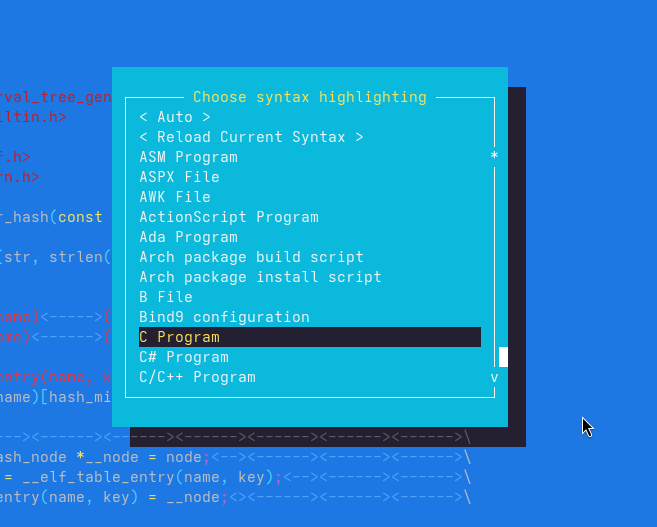
\includegraphics[width=0.7\linewidth,height=0.7\textheight]{image/34.png}

}

\caption{Цветовыделение синтаксиса}

\end{figure}%

\chapter{Вывод}\label{ux432ux44bux432ux43eux434}

В данной работе мы ознакомились с инструментами командной оболочки
Midnight Commander. Приобрели навыки практической работы по просмотру
каталогов и файлов

\chapter{Контрольные
вопросы}\label{ux43aux43eux43dux442ux440ux43eux43bux44cux43dux44bux435-ux432ux43eux43fux440ux43eux441ux44b}

\begin{enumerate}
\def\labelenumi{\arabic{enumi}.}
\item
  Какие режимы работы есть в mc? Охарактеризуйте их. Ответ: В командной
  оболочке mc есть два режима Информация и Дерево. В режиме Информация
  на панель выводятся сведения о файле и текущей файловой системе,
  расположенных на активной панели. В режиме Дерево на одной из панелей
  выводится структура дерева каталогов. Управлять режимами отображения
  панелей можно через пункты меню mc
\item
  Какие операции с файлами можно выполнить как с помощью команд shell,
  так и с помощью меню mc? Привести несколько примеров. Ответ: Командные
  интерпретатор Shell и оболочка Midnight Commander имеют похожую
  структуру и многие одинаковые команды можно выполнить в обоих
  оболочках вот некоторые из них
\end{enumerate}

\begin{enumerate}
\def\labelenumi{\alph{enumi})}
\tightlist
\item
  Системная информация
\item
  Поиск
\item
  Копирование
\end{enumerate}

\begin{enumerate}
\def\labelenumi{\arabic{enumi}.}
\setcounter{enumi}{2}
\tightlist
\item
  Опишите структуру меню левой панели mc, дайте характеристику командам.
  Ответ: Меню левой панели mc представляет собой следующую конструкцию:
\end{enumerate}

Где подпункты меню a) Список файлов показывает файлы в домашнем
каталоге. b) Быстрый просмотр позволяет выполнить быстрый просмотр
содержимого панели.\\
с) Информация позволяет посмотреть информацию о файле или каталоге d)
Командная оболочка Midnight Commander В меню каждой (левой или правой)
панели можно выбрать Формат списка: стандартный, ускоренный, расширенный
и определённый пользователем. e) Порядок сортировки позволяет задать
критерии сортировки при выводе списка файлов и каталогов: без
сортировки, по имени, расширенный, время правки, время доступа, время
изменения атрибута, размер, узел.

\begin{enumerate}
\def\labelenumi{\arabic{enumi}.}
\setcounter{enumi}{3}
\tightlist
\item
  Опишите структура меню Файл mc и дайте характеристику командам. Ответ:
  Меню Фаил mc представляет собой следующую конструкцию:
\end{enumerate}

Где подпункты меню a) Просмотр ( F3 ) позволяет посмотреть содержимое
текущего файла без возможности редактирования. b) -- Просмотр вывода
команды ( М + ! ) функция запроса команды с параметрами. c) Правка ( F4
) открывает текущий (или выделенный) файл для его редактирования. d)
Копирование ( F5 ) осуществляет копирование одного или нескольких файлов
или каталогов в указанное пользователем во всплывающем окне место. e)
Права доступа ( Ctrl-x c ) позволяет изменить права доступа к одному или
нескольким файлам или каталогам. f) Права доступа на файлы и каталоги g)
Жёсткая ссылка ( Ctrl-x l ) позволяет создать жёсткую ссылку к текущему
(или выделенному) файлу1 . h) Символическая ссылка ( Ctrl-x s ) ---
позволяет создать символическую ссылку к текущему файлу . i) Владелец
группы ( Ctrl-x o ) позволяет задать владельца и имя группы для одного
или нескольких файлов или каталогов. j) Права (расширенные) позволяет
изменить права доступа и владения для одного или нескольких файлов или
каталогов. k) Переименование ( F6 ) позволяет переименовать один или
несколько файлов или каталогов. l) Создание каталога ( F7 ) позволяет
создать каталог. m) Удалить ( F8 ) позволяет удалить один или несколько
файлов или каталогов. n) Выход ( F10 ) завершает работу mc.

5 Опишите структура меню Команда mc, дайте характеристику командам
Ответ: Ответ: Меню Команда mc представляет собой следующую конструкцию:

Где подпункты меню a) Дерево каталогов отображает структуру каталогов
системы. b) Поиск файла выполняет поиск файлов по заданным параметрам.\\
c) Переставить панели меняет местами левую и правую панели. d) Сравнить
каталоги ( Ctrl-x d ) сравнивает содержимое двух каталогов. e) Размеры
каталогов отображает размер и время изменения каталога (по умол- чанию в
mc размер каталога корректно не отображается). f) История командной
строки выводит на экран список ранее выполненных в оболочке команд. g)
Каталоги быстрого доступа ( Ctrl-~) при вызове выполняется быстрая смена
текущего каталога на один из заданного списка. h) Восстановление файлов
позволяет восстановить файлы на файловых систе- мах ext2 и ext3. i)
Редактировать файл расширений позволяет задать с помощью определённого
синтаксиса действия при запуске файлов с определённым расширением
(напри- мер, какое программного обеспечение запускать для открытия или
редактирова- ния файлов с расширением .c или .cpp). j) Редактировать
файл меню позволяет отредактировать контекстное меню поль- зователя,
вызываемое по клавише F2 . k) Редактировать файл расцветки имён
позволяет подобрать оптимальную для пользователя расцветку имён файлов в
зависимости от их типа.

\begin{enumerate}
\def\labelenumi{\arabic{enumi}.}
\setcounter{enumi}{5}
\tightlist
\item
  Опишите структура меню Настройки mc, дайте характеристику командам
  Ответ: Меню Настройки mc представляет собой следующую конструкцию:
\end{enumerate}

Где подпункты меню a) Конфигурация позволяет скорректировать настройки
работы с панелями. b) Внешний вид и Настройки панелей определяет
элементы, отображаемые при вызове mc, а также цветовое выделение. c)
Биты символов задаёт формат обработки информации локальным термина- лом.
d) Подтверждение позволяет установить или убрать вывод окна с запросом
подтверждения действий при операциях удаления и перезаписи файлов, а
также при выходе из программы. e) Распознание клавиш диалоговое окно
используется для тестирования функциональных клавиш, клавиш управления
курсором и прочее. f) Виртуальные ФС настройки виртуальной файловой
системы: тайм-аут, пароль и прочее.

\begin{enumerate}
\def\labelenumi{\arabic{enumi}.}
\setcounter{enumi}{6}
\tightlist
\item
  Назовите и дайте характеристику встроенным командам mc. Ответ: В
  командную оболочку mc встроены стандартные команды. Вот некоторые из
  них.
\end{enumerate}

\begin{enumerate}
\def\labelenumi{\alph{enumi})}
\tightlist
\item
  F1 Вызов контекстно-зависимой подсказки.
\item
  F2 Вызов пользовательского меню с возможностью создания and/or.
\item
  F3 Просмотр содержимого файла, на который указывает подсветка в
  активной панели.
\item
  F4 Вызов встроенного в mc редактора для изменения содержания файла, на
  который указывает подсветка в активной панели.
\item
  F5 Копирование одного или нескольких файлов, отмеченных в первой
  (активной) панели, в каталог, отображаемый на второй панели.
\item
  F6 Перенос одного или нескольких файлов, отмеченных в первой панели, в
  каталог, отображаемый на второй панели.
\item
  F7 Создание подкаталога в каталоге, отображаемом в активной панели.
\item
  F8 Удаление одного или нескольких файлов, отмеченных в первой панели
  файлов.
\item
  Вызов меню mc.
\item
  F10 Выход из mc.
\end{enumerate}

8 Назовите и дайте характеристику командам встроенного редактора mc.
Ответ: В редактор mc встроено немало команд. Вот некоторые из них. a)
Ctrl+y удалить строку. b) Ctrl+u отмена последней операции. c) Ins
вставка/замена. d)F7 поиск. d)Shift+F7 повтор последней операции поиска.
e) F4 замена файла. f) F3 первое нажатие начало выделения, второе это
окончание выделения. g) F5 копировать выделенный фрагмент F6 переместить
выделенный фрагмент. h) F8 удалить выделенный фрагмент. i) F2 записать
изменения в файл. j) F10 выйти из редактора.

\begin{enumerate}
\def\labelenumi{\arabic{enumi}.}
\setcounter{enumi}{8}
\item
  Дайте характеристику средствам mc, которые позволяют создавать меню,
  определяемые пользователем. Ответ: Один из четырех форматов списка в
  Midnight Commander -Пользовательский определённый самим пользователем
  позволяет ему редактировать меню любого из двух списков. А меню
  пользователя -- это меню, состоящее из команд, определенных
  пользователем. При вызове меню используется файл
  \textasciitilde/.mc.menu. Если такого файла нет, то по умолчанию
  используется системный файл меню /usr/lib/mc/mc.menu. Все строки в
  этих файлах , начинающиеся с пробела или табуляции, являются
  командами, которые выполняются при выборе записи.
\item
  Дайте характеристику средствам mc, которые позволяют выполнять
  действия, определяемые пользователем, над текущим файлом Ответ: Когда
  мы выделяем файл не являющегося исполняемым, Midnight Commander
  сравнивает расширение выбранного файла с расширениями, прописанными в
  «файле расширений» \textasciitilde/mc.ext. Если в файле расширений
  найдется подраздел, задающий процедуры обработки файлов с данным
  расширением, то обработка файла производится в соответствии с
  заданными в этом подразделе командами и файлами:
\end{enumerate}

\begin{enumerate}
\def\labelenumi{\alph{enumi})}
\tightlist
\item
  файл помощи для MC. /usr/lib/mc.hlp
\item
  файл расширений, используемый по умолчанию. /usr/lib/mc/mc.ext
\item
  файл расширений, конфигурации редактора. \$HOME/.mc.ext
\item
  системный инициализационный файл. /usr/lib/mc/mc.ini
\item
  фаил который содержит основные установки. /usr/lib/mc/mc.lib
\item
  инициализационный файл пользователя. Если он существует, то системный
  файл mc.ini игнорируется. \$HOME/.mc.ini
\item
  этот файл содержит подсказки, отображаемые в нижней части экрана.
  /usr/lib/mc/mc.hint
\item
  системный файл меню MC, используемый по умолчанию. /usr/lib/mc/mc.menu
\item
  файл меню пользователя. Если он существует, то системный файл меню
  игнорируется. \$HOME/.mc.menu
\item
  инициализационный файл пользователя. Если он существует, то системный
  файл mc.ini игнорируется. \$HOME/.mc.tree
\end{enumerate}


\printbibliography



\end{document}
